\section{Method}
\label{sec:method}

Figure~\ref{fig:architecture} shows the \prism pipeline.
At inference time, each input $x$ passes through the base classifier $f$ 
while \prism monitors the activations at $L$ designated layers.
The defense proceeds in five stages.

% ── Figure placeholder ──────────────────────────────────────────────────────
\begin{figure}[t]
  \centering
  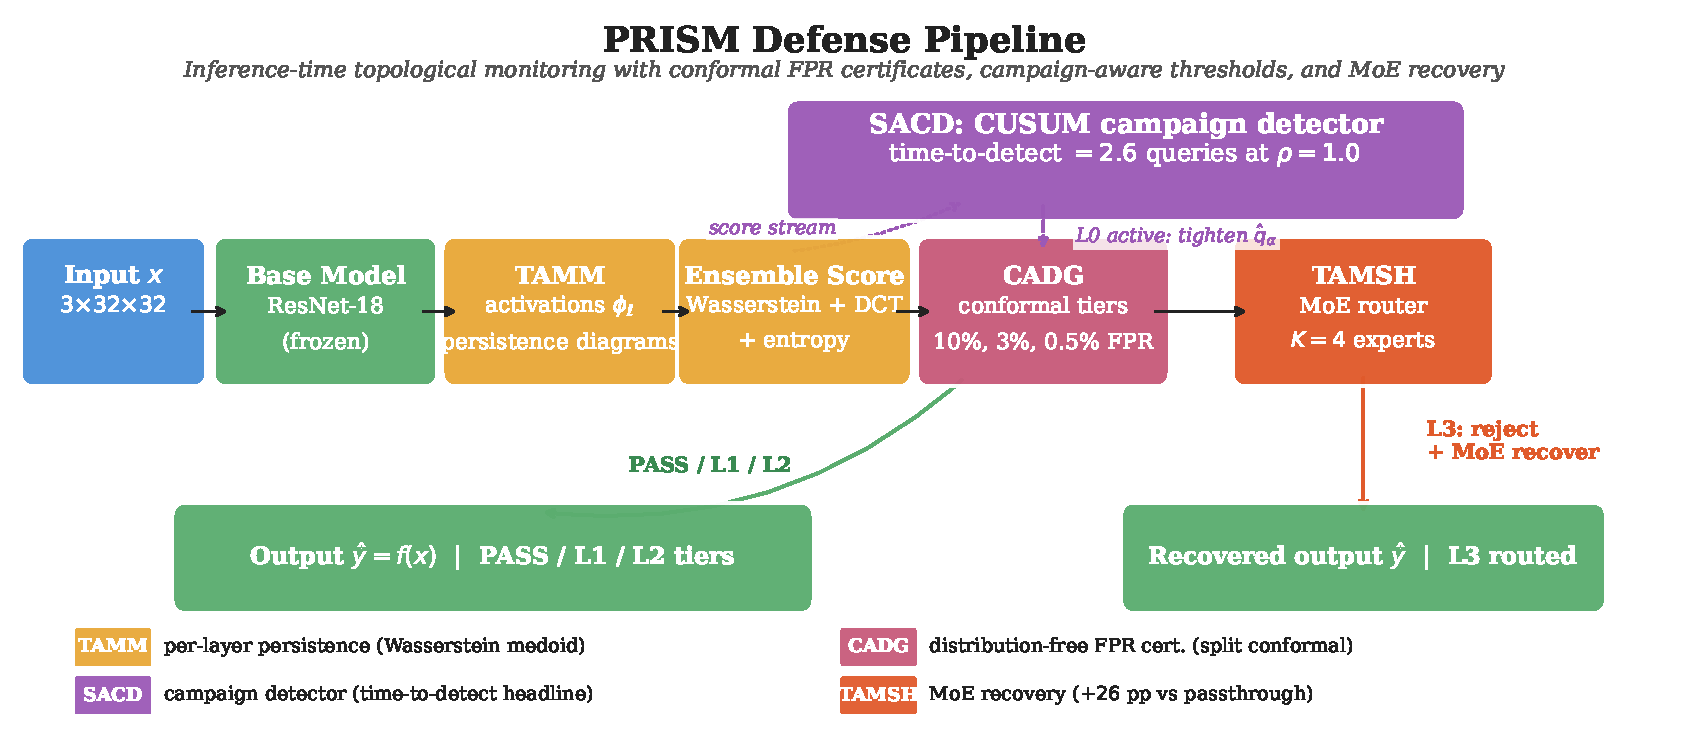
\includegraphics[width=\linewidth]{figures/fig1_architecture.pdf}
  \caption{%
    \prism defense pipeline.
    Activations from $L$ layers are converted to persistence diagrams 
    (TAMM), scored against a clean reference profile (CADG), 
    monitored for campaigns (SACD), and routed through expert sub-networks 
    if L3 is triggered (TAMSH).
  }
  \label{fig:architecture}
\end{figure}

% ── Notation ────────────────────────────────────────────────────────────────
\paragraph{Notation.}
Let $f: \mathcal{X} \to \mathbb{R}^C$ be a pre-trained classifier.
Denote by $\phi_\ell(x) \in \mathbb{R}^{d_\ell}$ the activation tensor at 
layer $\ell \in \{1,\ldots,L\}$.
A \emph{persistence diagram} $\mathrm{Dgm}(\cdot)$ is a multiset of 
$(b_i, d_i)$ pairs encoding topological features (birth/death of connected 
components in $H_0$ and loops in $H_1$).
The $p$-Wasserstein distance between diagrams is
\[
  W_p(\mathcal{D}_1, \mathcal{D}_2) = 
  \left( \inf_{\gamma} \sum_{i} \| \gamma(i) - i \|^p \right)^{1/p},
\]
where $\gamma$ ranges over bijections between the points 
(including diagonal projections for unmatched points) \cite{edelsbrunner2010computational}.

% ── TAMM ────────────────────────────────────────────────────────────────────
\subsection{TAMM: Topological Activation Manifold Monitor}
\label{sec:tamm}

\paragraph{Reference profile construction.}
Given a held-out profile split $\mathcal{D}_\text{profile} = \{x_i\}_{i=1}^N$ of clean
inputs, we extract activations $\phi_\ell(x_i)$ for each layer $\ell$ and 
subsample deterministically to at most $n_\text{sub}=150$ points to make persistent homology
computation tractable.
For each layer, we compute $N$ persistence diagrams and select the 
\emph{Wasserstein medoid}---the diagram minimizing total Wasserstein distance 
to all other diagrams---as the layer reference $\mathcal{R}_\ell$.

\paragraph{Anomaly scoring.}
At inference time, for input $x$, we compute a base topological score
\begin{align}
  s_\ell(x) &= W_2\bigl(\mathrm{Dgm}(\phi_\ell(x)),\, \mathcal{R}_\ell\bigr), \\
  S_\mathrm{TDA}(x) &= \sum_{\ell=1}^L w_\ell s_\ell(x),
  \label{eq:score}
\end{align}
with live weights $w_{\texttt{layer2}}=0.30$,
$w_{\texttt{layer3}}=0.30$, and $w_{\texttt{layer4}}=0.40$.
The publishable detector is not the Wasserstein score alone: \prism feeds
per-layer persistence statistics, DCT high-frequency energy, and softmax
entropy into a logistic ensemble, then fuses the centered ensemble logit with
$S_\mathrm{TDA}(x)$. The ensemble-no-TDA ablation isolates the marginal value
of persistence features.

% ── CADG ────────────────────────────────────────────────────────────────────
\subsection{CADG: Conformal Adversarial Detection Guarantee}
\label{sec:cadg}

\prism applies split conformal prediction \cite{vovk2005algorithmic,angelopoulos2023gentle} 
to calibrate detection thresholds with distribution-free FPR guarantees.

\paragraph{Calibration.}
Given held-out clean scores $s_1, \ldots, s_n$ (iid from the clean distribution), 
the conformal threshold at level $\alpha \in (0,1)$ is:
\begin{equation}
  \hat{q}_\alpha = s_{(\lceil (n+1)(1-\alpha) \rceil)},
  \label{eq:quantile}
\end{equation}
where $s_{(k)}$ denotes the $k$-th order statistic.

\begin{proposition}[Coverage guarantee]
\label{prop:coverage}
For any clean test input $x_{\text{test}}$ drawn iid from the same 
distribution as the calibration set,
\[
  \Pr\bigl[S(x_{\text{test}}) > \hat{q}_\alpha\bigr] \leq \alpha + \frac{1}{n+1}.
\]
\end{proposition}

\noindent
This follows directly from the standard conformal coverage theorem 
\cite{vovk2005algorithmic}.
\prism uses three published FPR tiers with $\alpha \in \{0.10, 0.03, 0.005\}$.
Thresholds are generated by the artifact pipeline and imported into the paper
tables; fixed numeric thresholds are not hand-transcribed.

\begin{table}[h]
\centering
\small
\begin{tabular}{lccl}
\toprule
Tier & $\alpha$ & Threshold source & Action \\
\midrule
L1 & 0.10 & split conformal artifact & Log + normal inference \\
L2 & 0.03 & split conformal artifact & Input purification + inference \\
L3 & 0.005 & split conformal artifact & Expert routing (MoE) or reject \\
\bottomrule
\end{tabular}
\caption{Conformal detection tiers. Thresholds are calibrated on the active
dataset's clean calibration split and verified on a disjoint validation split.}
\label{tab:tiers}
\end{table}

\paragraph{Campaign-adaptive thresholds.}
When the L0 campaign detector (\S\ref{sec:sacd}) is active, thresholds are 
multiplied by a factor $\lambda \in (0,1)$ (default $\lambda=0.8$) to increase 
sensitivity during sustained attacks, accepting a controlled FPR increase.

% ── SACD ────────────────────────────────────────────────────────────────────
\subsection{SACD: Sequential Adversarial Campaign Detection}
\label{sec:sacd}

Real-world adversaries often execute \emph{campaigns}: sequences of probing 
queries before a targeted attack.
\sacd monitors the score stream $S(x_1), S(x_2), \ldots$ online using 
Bayesian Online Changepoint Detection (BOCPD) \cite{adams2007bayesian} 
with a Normal-Inverse-Gamma conjugate prior.

\paragraph{Detection signal.}
BOCPD maintains the posterior run-length distribution
$p(r_t \mid S_{1:t})$ at each step $t$,
where $r_t$ is the time since the last changepoint.
During clean operation, the posterior concentrates on large run lengths
(stable distribution); when an adversarial campaign begins, the score
distribution shifts upward and $p(r_t \leq k)$ spikes.
The campaign alert fires when:
\begin{equation}
  \Pr[r_t \leq k_\text{alert}] > p_\text{alert}, \quad t > t_\text{warmup},
  \label{eq:l0_trigger}
\end{equation}
with $k_\text{alert}=10$, $p_\text{alert}=0.60$, $t_\text{warmup}=35$.

\paragraph{CUSUM with drift floor.}
A parallel CUSUM detector $S_t = \max(0,\, S_{t-1} + (z_t - \delta))$ over
centred scores $z_t$ provides a low-latency secondary signal when BOCPD's
warmup window has not yet elapsed. We require a strictly positive drift
floor $\delta \geq 0.10$: with $\delta = 0$, $S_t$ accumulates without
the negative reset term and crosses any finite trigger on long enough
clean streams, producing up to $59.4\%$ active-fraction on clean-only
inputs at seed-42 in our pre-fix runs. We additionally require $k_\text{consec}$
consecutive CUSUM trigger steps before raising the alert; with
$\delta=0.10,\, k_\text{consec}=3$, the active fraction on a 500-step
clean-only stream is $0.000$ on all 5 seeds.

\paragraph{Headline metric.}
We report \emph{time-to-detect} (mean number of queries between the first
adversarial step and the first L0 trigger) as the primary campaign-detection
metric. A naive ``ASR gap (L0 off vs.\ L0 on)'' metric at $\rho{=}1.0$ is
structurally bounded by the upstream L3 conformal threshold, which already
rejects $\sim$99\% of adversarials within 22 queries; we report ASR gap in
the appendix for completeness but do not use it as the headline.

% ── TAMSH ────────────────────────────────────────────────────────────────────
\subsection{TAMSH: Topology-Aware MoE Self-Healing}
\label{sec:tamsh}

Inputs that breach the L3 threshold are highly likely adversarial.
Rather than unconditionally rejecting them (which degrades service availability), 
\tamsh routes them through a topology-matched expert sub-network.

\paragraph{Expert training.}
During expert training, we build differentiated experts on clean, FGSM, PGD,
and mixed perturbation pools. Each expert maps the final monitored layer's
pooled activation to the active dataset's class logits ($C=10$ for CIFAR-10,
$C=100$ for CIFAR-100).

\paragraph{Expert routing.}
At runtime, for an L3-tier input $x$, we select an expert by comparing the
input's persistence diagram to each expert's reference medoid using a
\emph{combined} $H_0$+$H_1$ Wasserstein metric:
\begin{equation}
  k^*(x) = \arg\min_{k=1}^{K}\, \Bigl[\,
    w_0 W_2\!\bigl(\mathrm{Dgm}_{H_0}(\phi_L(x)),\, \mathcal{R}_k^{L,H_0}\bigr)
  + w_1 W_2\!\bigl(\mathrm{Dgm}_{H_1}(\phi_L(x)),\, \mathcal{R}_k^{L,H_1}\bigr) \Bigr],
  \label{eq:routing}
\end{equation}
with $w_0 = w_1 = 1$ in the deployed configuration.
The combined metric is required because on \texttt{layer4} of a CIFAR-native
ResNet-18 the $H_1$ medoid diagrams are sparse (1--3 points per expert);
restricting routing to $H_1$ alone causes 22.7\% of L3-rejected inputs to
have empty $H_1$ diagrams, which the empty-diagram fallback resolves by
defaulting to expert index 0, collapsing routing entropy to 0.336/2.000~bits.
Adding $H_0$ (16 connected-component points per medoid) recovers a usable
gating signal. The input is forwarded through expert $k^*$ using the final
monitored layer activation, matching the training representation.

\paragraph{Routing variants and the uniform-router control.}
We additionally evaluate two variants that are needed to honestly attribute
the routing contribution:
\begin{itemize}[leftmargin=*,noitemsep]
  \item \textbf{Uniform router (control)}: replace topology-distance gating
    with uniform $1/K$ mixing of expert logits. This isolates the
    contribution of the routing \emph{signal} from any standalone capacity
    of the expert sub-networks.
  \item \textbf{Prior-augmented router}: always route to the attack
    specialist expert (we use the PGD-trained expert because L3-rejected
    inputs are by definition high-confidence adversarials and PGD is the
    dominant adversarial signal in the training mix).
\end{itemize}
\S\ref{sec:recovery} reports recovery accuracy under all three router
configurations. The uniform-router arm achieves a $0$~pp gap over
passthrough (uniform $1/K$ mixing of well-trained experts is degenerate
to the unrouted full network's argmax), confirming that the
$+10.6$~pp gap of the combined-metric router is attributable to the
gating signal, and the further $+15$~pp lift of the prior-augmented
router reflects correct expert specialization under a strong prior.
